\documentclass[a4paper,12pt]{article}

%%%%%%%%%%%%%%%%%%%%%%%%%%%%%%%%%%%%%%%%%%%%%%%%
% Packages
%%%%%%%%%%%%%%%%%%%%%%%%%%%%%%%%%%%%%%%%%%%%%%%%

\usepackage[right=2.5cm, left=2.5cm, top=2.5cm, bottom=2.5cm]{geometry} 
\usepackage[portuguese]{babel}
\usepackage[T1]{fontenc}
\usepackage[utf8]{inputenc}
\usepackage{url}
\usepackage{hyperref}
\Urlmuskip=0mu  plus 10mu

% no indentation
%\usepackage{setspace}
%\setlength{\parindent}{0in}

\usepackage{graphicx} 
\usepackage{float}
\usepackage{xcolor}

\usepackage{mathtools}
\usepackage{amssymb, amsthm}
\usepackage{cancel}

% headers
\usepackage{fancyhdr}

%%%%%%%%%%%%%%%%%%%%%%%%%%%%%%%%%%%%%%%%%%%%%%%%
% Proper definitions
%%%%%%%%%%%%%%%%%%%%%%%%%%%%%%%%%%%%%%%%%%%%%%%%
\newcommand{\R}{\mathbb{R}}
\newcommand{\B}{\mathcal{B}}
\newcommand{\sur}{\mathcal{S}}

\newtheoremstyle{exer}{}{}{\color{blue}}{}{\color{blue}\bfseries}{}{ }{}
\theoremstyle{exer}
\newtheorem{exercise}{Exercício}

\theoremstyle{definition}
\newtheorem{solution}{Solução}
\newtheorem{definition}{Definição}

\theoremstyle{plain}
\newtheorem{remark}{Observação}



%%%%%%%%%%%%%%%%%%%%%%%%%%%%%%%%%%%%%%%%%%%%%%%%
% Header (and Footer)
%%%%%%%%%%%%%%%%%%%%%%%%%%%%%%%%%%%%%%%%%%%%%%%%

\pagestyle{fancy} 
\fancyhf{}

\lhead{\footnotesize CS: Lista 8}
\rhead{\footnotesize Prof. Asla e Mon. Lucas} 
\cfoot{\footnotesize \thepage} 


\begin{document}

%%%%%%%%%%%%%%%%%%%%%%%%%%%%%%%%%%%%%%%%%%%%%%%%
% Title section of the document
%%%%%%%%%%%%%%%%%%%%%%%%%%%%%%%%%%%%%%%%%%%%%%%%

\thispagestyle{empty} 

\begin{tabular*}{0.95\textwidth}{l @{\extracolsep{\fill}} r} 
    {\large \bf Curvas e Superfícies 2021.1} &  \\
    Escola de Matemática Aplicada, Fundação Getulio Vargas &  \\
    Professora Asla Medeiros e Sá &  \\ 
    Monitor Lucas Machado Moschen & Entrega 14/06/2021\\
    \hline \\
\end{tabular*} 
\vspace*{0.3cm} 

\begin{center}
	{\Large \bf Lista 8}
	\vspace{2mm}
\end{center}  
\vspace{0.4cm}

\begin{exercise}
    Estudo do cilindro:
    \begin{enumerate}
    \item[(a)] Escolha uma parametrização de parte de uma superfície cilíndrica regular.
    \item[(b)] Desenhar, em software gráfico, as seções normais para um ponto da imagem da
    parametrização escolhida. Observe as direções em que as curvaturas das curvas
    definidas pela seção normal são máxima e mínima.
    \item[(c)] Defina uma aplicação normal de Gauss para a parametrização escolhida.
    \item[(d)] Calcule os coeficientes da primeira forma fundamental para um ponto da parametrização proposta.
    \item[(e)] Calcule a área coberta pela parametrização proposta por você.
    \item[(f)] Calcule os coeficientes da segunda forma fundamental para o mesmo ponto analisado anteriormente.
    \item[(g)] Calcule as curvaturas principais e as direções principais para os pontos escolhidos
    do cilindro.   
\end{enumerate}
\end{exercise}

\begin{solution}
    \begin{enumerate}
        \item[(a)] Considere a parametrização 
        $$\sigma(u,v) = (\cos(u),
        \sin(u), v), (u,v) \in (0,2\pi) \times (-1,1).$$ 
        \item[(b)] A solução está na figura \ref{fig:cylinder}. O arquivo
        geogebra pode ser encontrado no Github\footnote{\url{https://github.com/lucasmoschen/ta-sessions/tree/master/Curves_Surfaces/lists/list8}}.

        \begin{figure}[!ht]
            \centering
            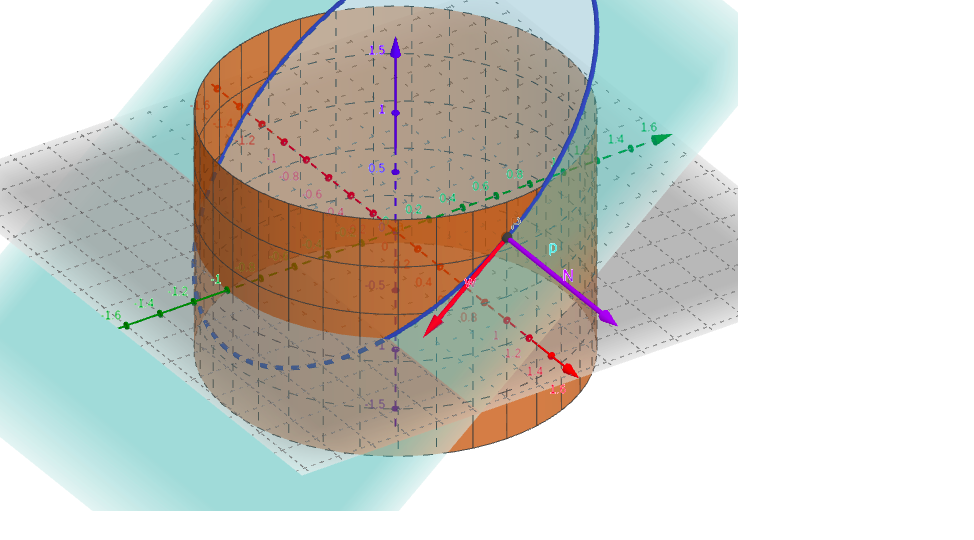
\includegraphics[width=0.6\textwidth]{images/cilindro.png}
            \caption{Cilindro em laranja. Vetor normal em roxo. Vetor do plano tangente em vermelho. Seção normal em azul.}
            \label{fig:cylinder}
        \end{figure}

        \item[(c)] Dado um ponto $p$, temos que 
        $$
        N \propto \sigma_u \times \sigma_v = (\cos(u), \sin(u), 0) \implies N(p) = \operatorname{proj}_p XY = \pi(p)
        $$
        \item[(d)] A primeira forma fundamental é dada por 
        $$
        E = ||\sigma_u||^2 = 1, F = \sigma_u\cdot\sigma_v = 0, G = ||\sigma_v||^2 = 1
        $$
        que pode ser escrita como 
        $$
        du^2 + dv^2
        $$
        \item[(e)] Nesse caso, observe que $EG - F^2 = 1$ e, portanto
        $$
        A = \int_{-1}^1\int_0^{2\pi} 1 du dv = 4\pi
        $$
        \item[(f)] A segunda forma fundamental é dada por 
        $$
        e = \sigma_{uu}\cdot N = -1, f = \sigma_{uv}\cdot N = 0, g = \sigma_{vv}\cdot N = 0
        $$
        que pode ser reescrita como 
        $$
        -du^2
        $$ 
        \item[(g)] Para calcular as curvaturas principais e direções
        principais, precisamos procurar os autovalores e autovetores do mapa
        de Weingarten. A matriz correspondente ao mapa é dada pelo produto
        matricial do inverso da primeira forma fundamental pela segunda forma
        fundamental, isto é, 
        $$
        \begin{bmatrix}
            1 & 0 \\ 0 & 1
        \end{bmatrix}^{-1}\begin{bmatrix}
            -1 & 0 \\ 0 & 0 
        \end{bmatrix} = \begin{bmatrix}
            -1 & 0 \\ 0 & 0 
        \end{bmatrix}
        $$
        que tem autovalores $0$ e $-1$ associados às direções $(0,1)$ e
        $(1,0)$, respectivamente. Observe que se o vetor normal fosse definido
        como $-N$, a curvatura principal $-1$ seria $+1$.
    \end{enumerate}
\end{solution}

\begin{exercise}
    Para o paraboloide hiperbólico dado pela parametrização $$X(u, v) = (u, v,
    v^2 - u^2), (u, v) \in \R^2,$$ faça:
    \begin{enumerate}
        \item[(a)] Desenhar, em software gráfico, as seções normais para um
        ponto do paraboloide. Observe as direções em que as curvaturas das curvas
        definidas pela seção normal são máxima e mínima. 
        \item[(b)] Calcule os coeficientes da segunda forma fundamental para o
        ponto $q = (0, 0)$.  
        \item[(c)] Calcule as curvaturas principais, a curvatura gaussiana e a
        curvatura média para esse ponto.
    \end{enumerate}
\end{exercise}

\begin{solution}
    \begin{enumerate}
        \item[(a)] O desenho está na figura abaixo \ref{fig:paraboloid}. O
        código está no Github. 
        
        \begin{figure}[!ht]
            \centering
            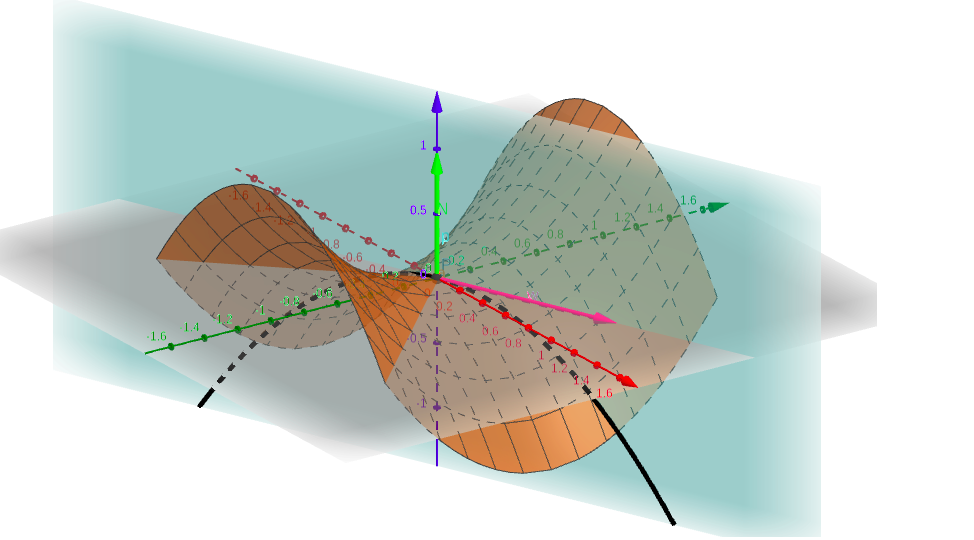
\includegraphics[width=0.6\textwidth]{images/paraboloide.png}
            \caption{Paraboloide em laranja. Vetor normal em verde. Vetor do plano tangente em rosa. Seção normal em preto.}
            \label{fig:paraboloid}
        \end{figure}
    \end{enumerate}

    \item[(b)] O vetor normal é dado por 
    $$
    N \propto \sigma_u \times \sigma_v = (2u, -2v, 1).
    $$
    Assim
    $$
    e = (0,0,-2)\cdot N = -\frac{2}{\sqrt{4u^2+4v^2+1}},
    $$
    $$
    f = 0,
    $$
    $$
    g = (0,0,2)\cdot N = \frac{2}{\sqrt{4u^2+4v^2+1}}
    $$
    No ponto $q$, isso vale $-2,0,2$, respectivamente. 

    \item[(c)] A primeira forma fundamental é dada por 
    $$
    E = ||\sigma_u||^2 = 4u^2 + 1, 
    $$
    $$
    F = \sigma_u \cdot \sigma_v = -4uv
    $$
    $$
    G = ||\sigma_v||^2 = 4v^2 + 1, 
    $$
    que em $q$ vale $1,0,1$ respectivamente. Logo a representação do mapa de
    Weingarten na base $\{X_u, X_v\}$ é 
    $$
    \begin{bmatrix}
        1 & 0 \\ 0 & 1
    \end{bmatrix}^{-1}\begin{bmatrix}
        -2 & 0 \\ 0 & 2 
    \end{bmatrix} = \begin{bmatrix}
        -2 & 0 \\ 0 & 2 
    \end{bmatrix}.
    $$
    As curvaturas principais são, portanto, $-2$ e $2$ (autovalores), a
    curvatura média é 0, e a curvatura Gaussiana é -4. 
\end{solution}

\begin{exercise}
    Para a sela de macaco dada pela parametrização 
    $$X(u, v) = (u, v,
    u^3- 3uv^2), (u, v) \in \R^2,$$ faça:
    \begin{enumerate}
        \item[(a)] Desenhar, em software gráfico, as seções normais para um ponto do sela.
        Observe as direções em que as curvaturas das cuvas definidas pela seção normal
        são máxima e mínima.
        \item[(b)] Calcule os coeficientes da segunda forma fundamental para o ponto $q =
        (0, 0)$.
        \item[(c)] Calcule as curvaturas principais, a curvatura gaussiana e a curvatura média para
        esse ponto.
    \end{enumerate}
\end{exercise}

\begin{solution}
    \begin{enumerate}
        \item[(a)] O desenho está na figura abaixo \ref{fig:sela}. O
        código está no Github. 
        
        \begin{figure}[!ht]
            \centering
            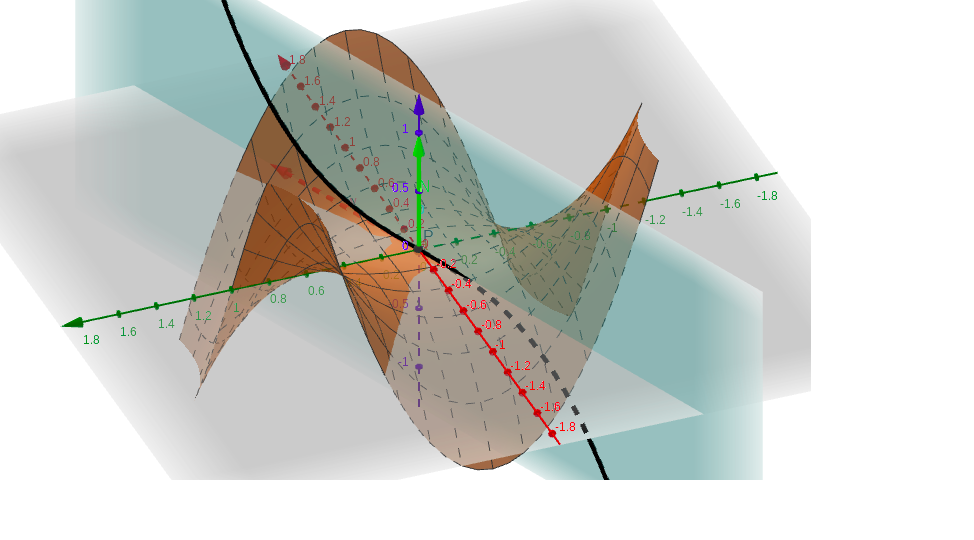
\includegraphics[width=0.6\textwidth]{images/sela.png}
            \caption{Sela em laranja. Vetor normal em verde. Vetor do plano tangente em rosa. Seção normal em preto.}
            \label{fig:sela}
        \end{figure}
    \end{enumerate}

    \item[(b)] O vetor normal é dado por 
    $$
    N \propto \sigma_u \times \sigma_v = (3v^2-3u^2 , 6uv, 1).
    $$
    Assim
    $$
    e = (0,0,6u)\cdot N = \frac{6u}{\sqrt{9v^4+18u^2v^2 + 9u^4+1}},
    $$
    $$
    f = (0,0,-6v)\cdot N = -\frac{6v}{\sqrt{9v^4+18u^2v^2 + 9u^4+1}},
    $$
    $$
    g = (0,0,-6u)\cdot N = -\frac{6u}{\sqrt{9v^4+18u^2v^2 + 9u^4+1}},
    $$
    No ponto $q$, isso vale $0,0,0$, respectivamente. 

    \item[(c)] A primeira forma fundamental é dada por 
    $$
    E = ||\sigma_u||^2 = 1 + (3u^2 - 3v^2)^2, 
    $$
    $$
    F = \sigma_u \cdot \sigma_v = 18uv^3 - 18u^3v
    $$
    $$
    G = ||\sigma_v||^2 = 1 + 16u^2v^2, 
    $$
    que em $q$ vale $1,0,1$ respectivamente. Logo a representação do mapa de
    Weingarten na base $\{X_u, X_v\}$ é 
    $$
    \begin{bmatrix}
        1 & 0 \\ 0 & 1
    \end{bmatrix}^{-1}\begin{bmatrix}
        0 & 0 \\ 0 & 0 
    \end{bmatrix} = \begin{bmatrix}
        0 & 0 \\ 0 & 0 
    \end{bmatrix}.
    $$
    As curvaturas principais são, portanto, $0$ e $0$ (autovalores), a
    curvatura média é 0, e a curvatura Gaussiana é 0 no ponto $q$. 
\end{solution}


\begin{exercise}
    Mostrar que planos são superfícies totalmente umbílicas.
\end{exercise}

\begin{solution}
    Seja o plano determinado pelos vetores $u$ e $v$ que passa pelo ponto
    $p_0$. Seja $p$ ponto desse plano. O vetor normal $N_p$ é dado por $u \times v$,
    contante para todo $p$. Assim o mapa de Weingarten (derivada do mapa $p
    \mapsto N_p$) é identicamente nulo.
    Em particular, os autovalores desse operator são 0, 0, iguais em todo
    ponto. Concluímos que o plano é totalmente umbílico. 
    
\end{solution}

\begin{exercise}
    Mostrar que esferas são superfícies totalmente umbílicas.
\end{exercise}

\begin{solution}
    Seja a esfera $\sur^2$ de centro $c$ e raio $r$. O mapa de Gauss é dado,
    para cada $p\in\sur^2$
    por 
    $$
    \mathcal{G}(p) = -\frac{1}{r}(p - c).
    $$
    Seja $v \in T_p\sur^2$ e $\gamma$ uma curva na esfera que passa em $t=0$ por $p$
    cuja derivada é $v$. Então, o mapa de Weingarten é 
    $$
    \mathcal{W}_{p,\sur^2}(v) = -D_p \mathcal{G} = -\frac{d}{dt} \mathcal{G} \circ \gamma(t)|_{t=0} = \frac{1}{r}\gamma'(t)|_{t=0} = \frac{1}{r}v,  
    $$
    e, portanto, o seu autovalor é $1/r$ com multiplicidade 2. Portanto $p$ é
    ponto umbilical e $\sur^2$ é totalmente umbílico.
\end{solution}

\begin{exercise}
    Detalhar a demonstração da página 4 das notas de aula (feitas também na
    aula em vídeo) que mostra que a curvatura das curvas definidas pelas
    seções normais coincide com a segunda forma fundamental. Isto é:
    $$
    k_{\alpha}(0) = \langle \alpha'', N(p) \rangle = \langle - dN_p(w), w \rangle = II_p
    $$
\end{exercise}

\begin{solution}
    Como o vetor $N(p)$ é ortogonal ao plano tangente, o plano $\Pi_{w, N}$
    gerado por $w \in T_pS$ e $N(p)$ são diferentes. Portanto $\Pi$ e $\sur$
    se intersectam
    transversalmente em $p$. Podemos portanto definir uma curva suave nessa
    intersecção em um aberto $U \subset \R^3$. Seja $\gamma : (-a,a) : U$ uma
    curva parametrizada por comprimento de arco tal que $\gamma(0) = p$ e seja
    a intersecção das superfícies. Teremos que $\gamma '(0) = w$. 

    Para todo ponto $t \in (-a,a)$, 
    $$
    \langle N(\gamma(t), \gamma'(t)) \rangle = 0 \overset{t=0}{\implies} \langle -DN_pw, w\rangle = \langle N(p), \gamma ''(0)\rangle,
    $$
    o que prova a afirmação.
\end{solution}


% \begin{thebibliography}{9}
%      \bibitem{pressley} 
%      Pressley, Andrew N. Elementary differential geometry. Springer Science \& Business Media, 2010.
% \end{thebibliography}

\end{document}